\section{窄读出条窄隙室——sTGC}
\label{chap:3_2}

在粒子物理实验中,人们需要对产生的粒子的状态进行记录才能进行后续的物理分析,这样粒子探测器就应运而生。粒子探测器经过精巧的设计,当粒子通过探测器的过程中与探测器中的物质发生反应,人们通过收集反应产生的次级粒子如光子、电子等信息来反推通过探测器的粒子的信息。粒子探测器的种类有很多,以与粒子发生相互作用的介质分类的话,粒子探测器可以分成气体探测器,液体探测器,固体探测器等几个大类。气体探测器因为其造价相对便宜、可以大规模制作等优点得到了广泛的应用,许多大型粒子物理实验如BES、STAR、ALICE等都将其用作主要的径迹探测器。在这一章当中主要介绍的小读出条窄隙室也是一种气体探测器。

在十九世纪七十年代之前,对于粒子径迹的探测手段主要是“照相”式的。以云室为例,当粒子通过充满了蒸汽的云室时和气体分子相互作用发生电离产生电子-离子对,这些电子-离子对作为凝结核使蒸汽凝成可见的雾珠。这样就使得不可见的粒子在穿过云室时留下可见的轨迹供人们进行分析。但这种“照相”式的探测手段的计数频率很低,极大地限制了实验的探测效率,人们希望能有电子学式的探测器,这样就可以极大地提高探测效率和径迹的信息收集能力。

在当时,正比计数器就已经被大量地应用在了射线的能谱测量当中,虽然可以通过将大量正比计数管组合在一起的方式来进行径迹探测,但是因为正比计数管本身的结构问题,这种解决方案的位置分辨有限且机械结构复杂。最开始人们曾经设想过是否可以在一个大的气体容器中平行地排列许多丝结构,但大多数人认为这样丝和丝之间会因为电容耦合效应导致信号传递到相邻的丝上,从而使得位置分辨变差。直到1968年,恰帕克(Georges Charpak)等人研究发现多丝结构可以按照预期设想工作并且获得很好的位置分辨,并据此发明了多丝正比室。恰帕克本人也因此获得了1992年的诺贝尔物理学奖。之后各种多丝室以及基于多丝室的探测器被不断地发明出来,成为了现在大型粒子物理实验的主力探测器。

窄读出条窄隙室(small-strip Thin Gap Chamber, sTGC)就是一种工作在饱和模式下的多丝室。sTGC的工作气体为55\%的二氧化碳和45\%的正戊烷组成的混合气体,阳极丝上加2900V的高压。
如图\ref{fig:sTGC}所示,STAR前向升级当中的窄隙室径迹探测器每一层由四个五边形的模块(Module)组成,四个不同的模块分别位于四个象限。以第一象限的A模块为第一块的话,之后每个象限的模块安置方式为A模块旋转(象限数-1)$*(-\frac{\pi}{2})$得到。每一个模块又由两个窄隙室组成。对于每一个窄隙室来说,两侧的阳极板背面均有读出条,其中一面读出条方向垂直于阳极丝,另一面读出条方向沿垂直于对角线方向,参见图\ref{fig:sTGC_chamber}。以第一象限的模组为例,从上到下的读出条方向分别为垂直于对角线方向,水平方向,竖直方向,垂直于对角线方向。从上往下各层的阳极丝和读出条方向如图\ref{fig:sTGC_chamber}中从左到右各图所示。

\begin{figure}[htb]
    \centering
    \begin{subfigure}[b]{0.3\textwidth}
        \centering
        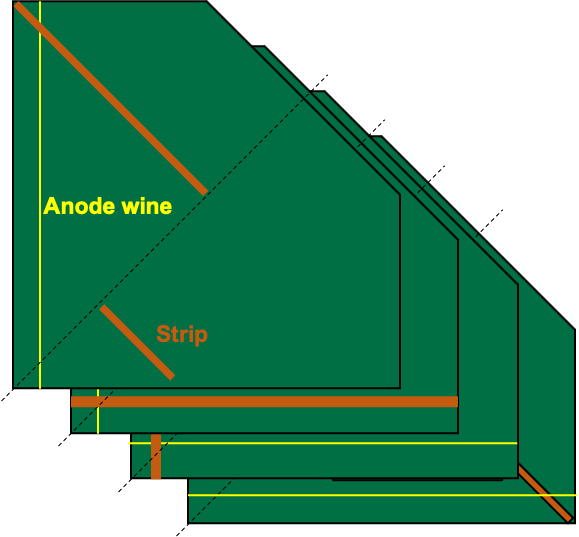
\includegraphics[width=\textwidth,clip]{figures/Chapter3/sTGC_Layers.png}
        \caption{}
        \label{fig:sTGC_Layers}
    \end{subfigure}
    \hfill
    \begin{subfigure}[b]{0.65\textwidth}
        \centering
        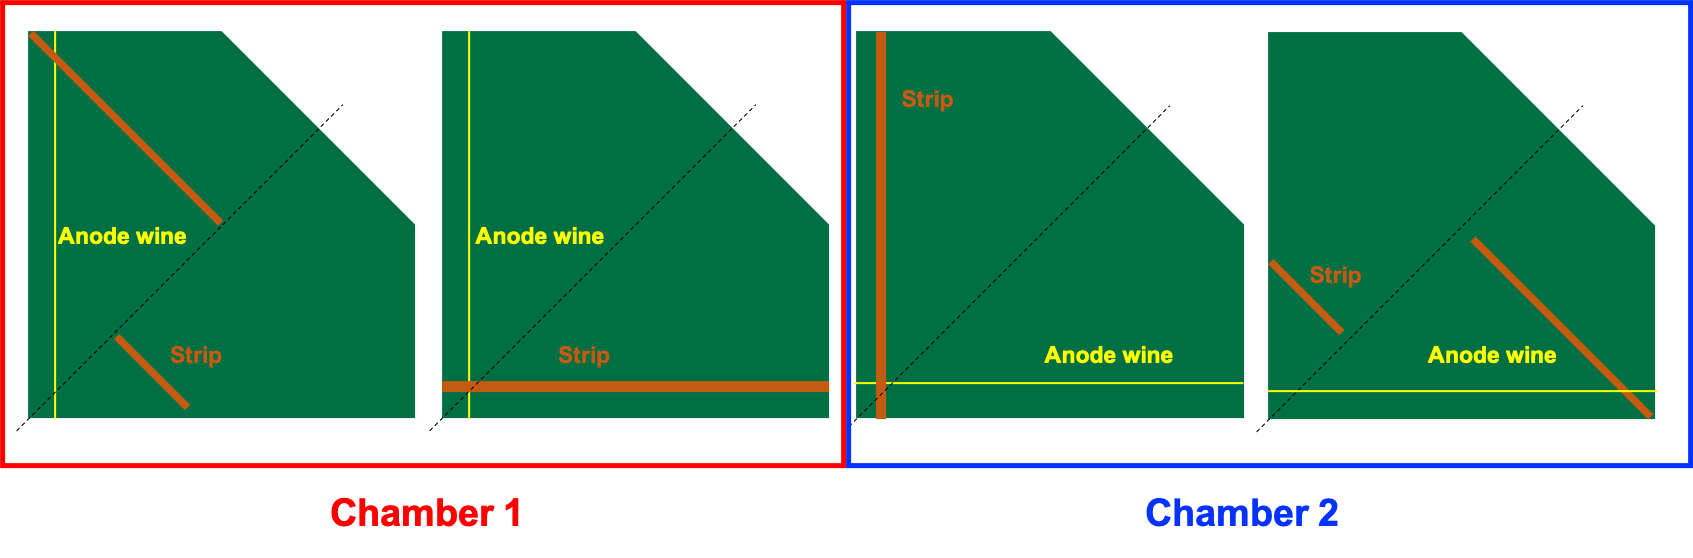
\includegraphics[width=\textwidth,clip]{figures/Chapter3/sTGC_chamber.png}
        \caption{}
        \label{fig:sTGC_chamber}
    \end{subfigure}
    \caption[sTGC 模组结构示意图]{\ref{fig:sTGC_Layers}为一个sTGC模组从上到下四层的阳极丝以及读出条的排列顺序。\ref{fig:sTGC_chamber}从左到右分别为图\ref{fig:sTGC_Layers}中的最上层到最后一层,其中前两层和后两层分属不同的室}
       \label{fig:sTGC_All_Layers}
\end{figure}

sTGC的侧视图如图\ref{fig:sTGC_sideview}所示。上下两层为覆盖有石墨的FR4板,涂有石墨的两面相对,作为探测器的阴极,相隔2.8mm。阳极丝位于两个FR4板的中间,距离两板各1.4mm。在阴极的背面是铜读出条(strip)。读出条宽2.7mm,读出条和读出条之间的间隙为0.5mm。读出条的长度根据读出条所在的位置不同有所不同,但大部分读出条的长度都远大于读出条的宽度。当粒子在窄隙室的阳极丝附近发生电离的时候发生雪崩过程,在读出条上产生感应信号,电子学可以收集这个感应信号并且将其转化成为数字信号储存起来,以供后期数据分析。
\begin{figure}[htb]
    \begin{center}
    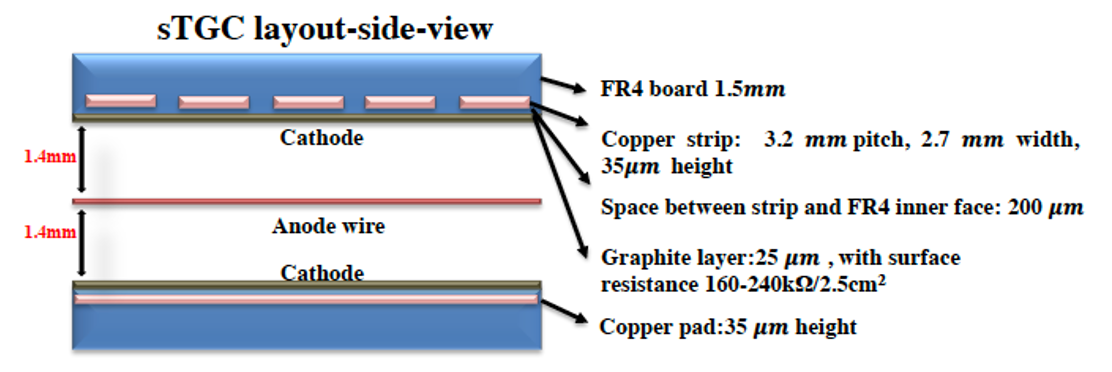
\includegraphics[width=0.7\textwidth,clip]{figures/Chapter3/sTGC_side_view.png}
    \end{center}
    \caption[sTGC侧视图]{sTGC侧视图}
    \label{fig:sTGC_sideview}
\end{figure}

当粒子通过阳极丝附近的时候,在工作气体中电离产生原初电子-离子对。电子开始向阳极丝附近漂移,而离子开始向阴极方向漂移。因为阳极丝上加有高压,电子在一个平均自由程内可以获得足够的能量使气体再次电离,从而在下次和气体分子碰撞的时候发生次级电离产生新的电子-离子对,次级电子-离子对又可以引发新的电离,从而使得电子-离子对的数目成指数形式增加。这个过程叫做雪崩过程。雪崩过程中电子会向阳极丝移动,产生感应信号后被阳极丝吸收。而离子因为质量较大,移动速度相比于电子来说较慢,会在阳极丝附近形成“阳离子鞘”并向阴极移动。这个过程中在阴极背面的读出条上产生感应信号。整个雪崩过程的示意图参见图\ref{fig:Avalanche}。电子学和读出条相连接,将这个感应信号读出。在收集到每个读出条的感应电荷信号之后,我们就可以通过电荷重心法来计算粒子通过窄隙室时发生电离的位置。计算公式为:

\begin{equation}
    \label{eq:center_of_gravity}
    x = \frac{\Sigma X_i*Q_i}{\Sigma Q_i} 
\end{equation}
其中$x$为重建出的电离发生的位置,$X_i$为产生感应信号的读出条的位置,$Q_i$为在对应的读出条上面产生的感应信号的大小。

\begin{figure}[htb]
    \begin{center}
    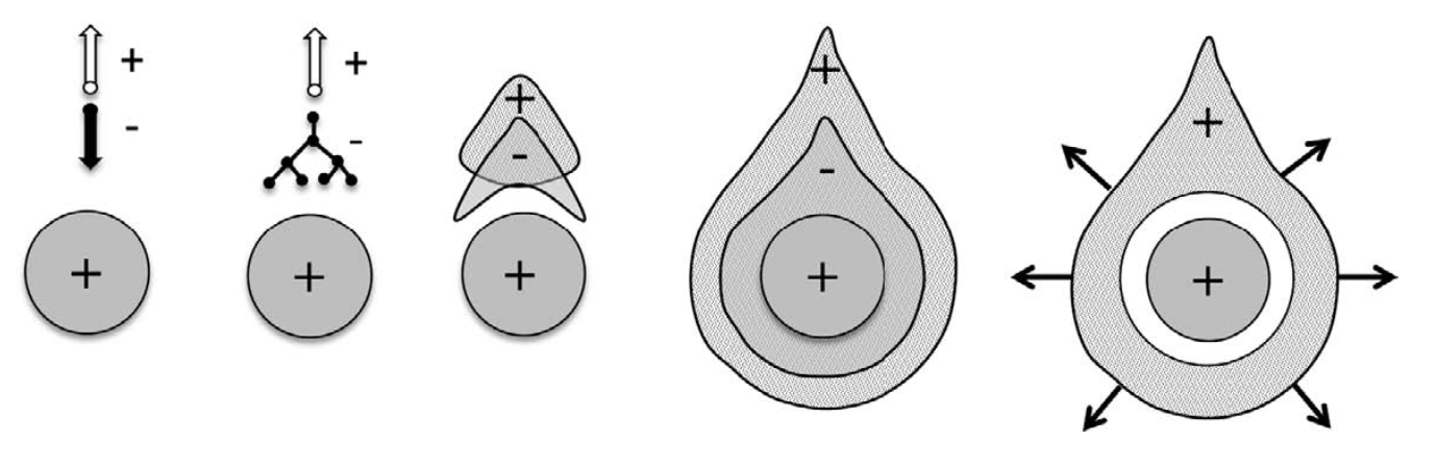
\includegraphics[width=0.7\textwidth,clip]{figures/Chapter3/Avalanche.png}
    \end{center}
    \caption[电子-离子对在阳极丝附近雪崩示意图]{电子-离子对在阳极丝附近雪崩示意图}
    \label{fig:Avalanche}
\end{figure}

从重建公式可以看出,对于沿着一个方向的读出条,我们只能重建出来和读出条垂直方向上的位置坐标。即沿着水平方向的读出条只能读出竖直方向上的位置坐标信息。这样四个读出层分别可以读出沿对角线方向、竖直方向、水平方向、沿对角线方向的一维位置坐标,如果需要得到二维的位置坐标我们需要对一维坐标进行配对,这就带来了ghost hit的问题。垂直于对角线方向的读出条和读出条本身的分组就是为了降低ghost hit的数目而设计的。关于这个问题将会在slow simulator和cluster finder一章进行详细讨论。